---

% 第 8 章 Poincaré 引理
\chapter{Poincaré 引理}

简而言之，Poincaré 引理如下.
\begin{theorem}[Poincaré 引理]\label{thm:8-1}
$\mathbb{R}^n$ 上的每个闭形式都是恰当的.
\end{theorem}
第 1 节详细介绍 Poincaré 引理及其含义. 严格地说，整个空间 $\mathbb{R}^n$ 并不是必需的. 证明对任何可缩为一点的星形区域都成立，但既然这不在证明中起本质作用，为了尽可能清晰，我们将简单地假设流形都是某个 $n\geq0$ 的 $\mathbb{R}^n$.

Poincaré 引理的证明基于归纳法. 如果你还没有上过数学证明课，我们将放慢速度、仔细地逐步进行，尽量把每一步解释清楚. 虽然这不是一门证明技巧课，但希望学完本章后你能对归纳证明是什么样子有一个好的认识. 第 2 节讲述所谓归纳证明的基础情形，第 3 节讲述证明的一般情形.

Poincaré 引理在一个称为 \newterm{de-rham-cohomology}{de Rham 上同调}{de Rham cohomology} 的数学分支中起着重要作用，该分支在附录 B 中简要介绍.

\section{Poincaré 引理导引}

Poincaré 引理断言 $\mathbb{R}^n$ 上的每个闭形式都是恰当的. 若 $d\alpha=0$，则微分形式 $\alpha$ 称为\newterm{closed}{闭的}{closed}. 若存在另一个微分形式 $\beta$ 使得 $\alpha=d\beta$，则微分形式 $\alpha$ 称为\newterm{exact}{恰当的}{exact}. 显然，若 $\alpha$ 是恰当的 $k$-形式，则 $\beta$ 必是 $(k-1)$-形式. 因此，Poincaré 引理还可以表述为：若 $\alpha$ 是 $\mathbb{R}^n$ 上满足 $d\alpha=0$ 的 $k$-形式，则存在某个 $(k-1)$-形式 $\beta$ 使得 $\alpha=d\beta$.

我们从考察某个流形 $M$ 上的恰当形式开始. 若一个 $k$-形式等于某个 $(k-1)$-形式的外微分，则称它是恰当的. 因此，所有恰当 $k$-形式的集合正是所有 $d\alpha$（其中 $\alpha$ 是 $(k-1)$-形式）的集合. 另一种说法是：恰当形式的集合是 $d:\Omega^{k-1}(M)\to\Omega^k(M)$ 在 $\Omega^{k-1}(M)$ 下的像. 图 \ref{fig:8-1} 用维恩图式的图解给出了映射 $d:\Omega^{k-1}(M)\to\Omega^k(M)$，以描绘恰当 $k$-形式.

\begin{figure}[htbp]
  \centering
  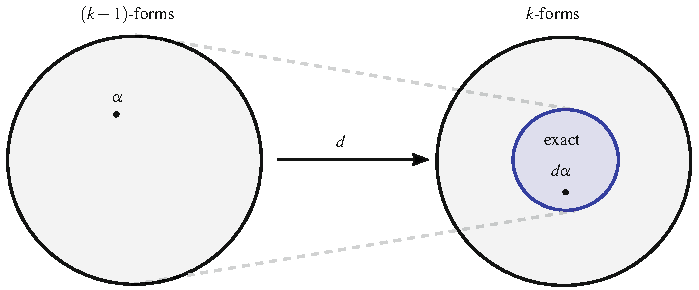
\includegraphics[width=0.829\linewidth]{images/vector/fig-8-1.pdf}
  \caption{用维恩图式图解说明的映射 $d:\Omega^{k-1}(M)\to\Omega^k(M)$. 恰当的 $k$-形式是 $\Omega^{k-1}(M)$ 在 $d$ 下的像}
  \label{fig:8-1}
\end{figure}

若 $M$ 上的 $k$-形式的外微分为零，即它等于零 $(k+1)$-形式，则称该 $k$-形式是闭的. 零 $(k+1)$-形式是每个把任意一组 $k+1$ 个向量都送到零的形式，它不应与零形式（即函数）混淆. 我们通常把任意点 $p$ 处的零 $k$-形式简单记为 $0$. 因此，所有闭 $k$-形式的集合就是满足 $d\alpha=0$ 的那些 $k$-形式 $\alpha$ 的集合. 另一种说法是：闭 $k$-形式的集合是零 $(k+1)$-形式在映射 $d:\Omega^k(M)\to\Omega^{k+1}(M)$ 下的原像. 图 \ref{fig:8-2} 用维恩图式给出了闭 $k$-形式的图像.

\begin{figure}[htbp]
  \centering
  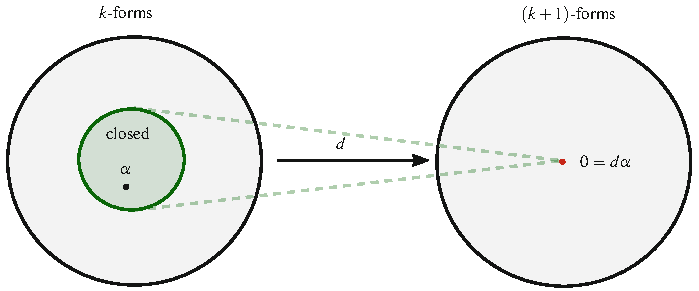
\includegraphics[width=0.829\linewidth]{images/vector/fig-8-2.pdf}
  \caption{用维恩图式图解说明的映射 $d:\Omega^k(M)\to\Omega^{k+1}(M)$. 闭的 $k$-形式是零 $(k+1)$-形式 $0$ 在 $d$ 下的原像}
  \label{fig:8-2}
\end{figure}

现在问题变成：闭 $k$-形式与恰当 $k$-形式之间有什么关系. 第一个猜测可能会沿着图 \ref{fig:8-3} 的思路，其中显示了若干种不同的可能性：
\begin{itemize}
  \item 恰当形式是闭形式的子集.
  \item 恰当形式与闭形式相同.
  \item 闭形式是恰当形式的子集.
  \item 闭形式与恰当形式互斥.
  \item 闭形式与恰当形式互不为对方的子集，但也不互斥.
\end{itemize}

\begin{figure}[htbp]
  \centering
  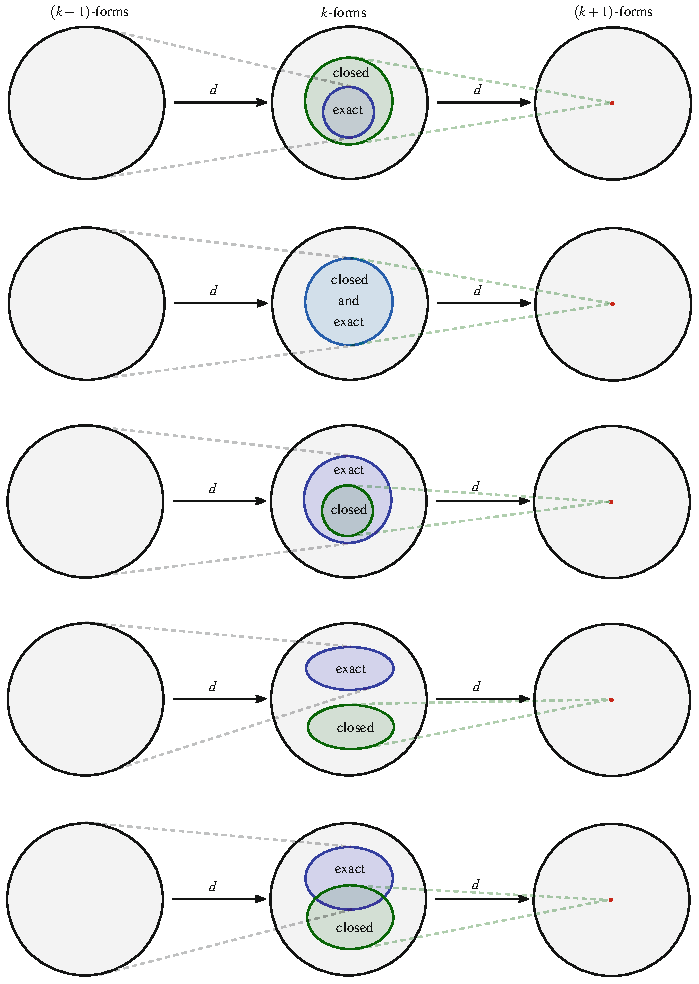
\includegraphics[width=0.885\linewidth]{images/vector/fig-8-3.pdf}
  \caption{闭 $k$-形式与恰当 $k$-形式之间可能存在的各种关系}
  \label{fig:8-3}
\end{figure}

然而，稍加思考几乎立刻就能排除最后三种可能性. 我们要做的只是认识到两个事实. 第一，每个恰当 $k$-形式都是某个 $(k-1)$-形式 $\alpha$ 的 $d\alpha$；第二，无论形式是什么，我们都有 $dd\alpha=0$. 这意味着每个恰当形式也是闭形式，从而排除了图 \ref{fig:8-3} 中的最后三种可能性. 剩下前两种可能性，即图 \ref{fig:8-4}.

\begin{figure}[htbp]
  \centering
  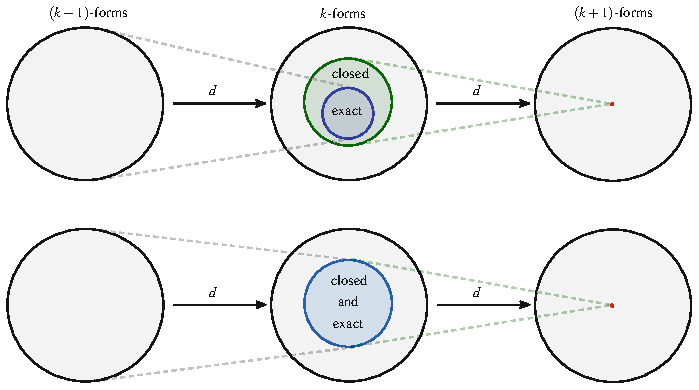
\includegraphics[width=0.907\linewidth]{images/vector/fig-8-4.pdf}
  \caption{恰当的 $k$-形式是闭 $k$-形式的子集（上方），还是与闭 $k$-形式相同（下方）？答案取决于流形 $M$}
  \label{fig:8-4}
\end{figure}

那么，图 \ref{fig:8-4} 中的两种可能性到底是哪一种呢？恰当形式是闭形式的子集，还是恰当形式与闭形式相同？结果表明，这个问题的答案取决于形式所在流形 $M$ 是什么. Poincaré 引理告诉我们，当流形是任意数 $n$ 的 $\mathbb{R}^n$ 时，恰当形式与闭形式相同. 但如果流形不是 $\mathbb{R}^n$，则情况未必如此. 称为 de Rham 上同调的数学分支考察 $M$ 上闭形式的集合与 $M$ 上恰当形式的集合相差多少，并利用这一信息来弄清底层流形 $M$ 的某些性质.

图 \ref{fig:8-5} 是一个交换图，展示了 $\mathbb{R}^n$ 上所有形式的空间，它向右和向下延伸到无穷. 显然，外微分给出映射序列
\[
\Omega^0(\mathbb{R}^n)\xrightarrow{\;d\;}\Omega^1(\mathbb{R}^n)\xrightarrow{\;d\;}\Omega^2(\mathbb{R}^n)\xrightarrow{\;d\;}\Omega^3(\mathbb{R}^n)\xrightarrow{\;d\;}\cdots
\]
对 $n=0,1,2,\ldots$ 的流形 $\mathbb{R}^n$ 成立. 映射 $K$ 是证明 Poincaré 引理所需的，将在下一节解释. 这给出交换图中的列. 映射
\[
Z:\Omega^k(\mathbb{R}^n)\to\Omega^k(\mathbb{R}^{n-1}),\qquad
C:\Omega^k(\mathbb{R}^n)\to\Omega^k(\mathbb{R}^{n+1}),
\]
其中 $k=1,2,\ldots$、$n=0,1,2,\ldots$，是我们证明 Poincaré 引理要用到的映射，它们也将在下一节引入. 在 Poincaré 引理的证明过程中，我们会反复参考这个交换图. 我们的目标是证明对 $n>0$ 的 $\mathbb{R}^n$ 上任意 $k>0$ 的闭 $k$-形式 $\alpha$ 都是恰当的. 换言之，我们要证明对每个满足 $d\alpha=0$ 的 $\alpha\in\Omega^k(\mathbb{R}^n)$，都存在 $\beta\in\Omega^{k-1}(\mathbb{R}^n)$ 使得 $\alpha=d\beta$. 实际上，我们不会显式地求出这个 $\beta$，而是对 $n$ 使用归纳法. 也就是说，如果我们知道它对 $\mathbb{R}^n$ 上的 $k$-形式成立，那么我们就能证明它对 $\mathbb{R}^{n+1}$ 成立. 图 \ref{fig:8-6} 给出了图 \ref{fig:8-5} 中交换图的列的维恩图式表示.

\begin{figure}[htbp]
  \centering
  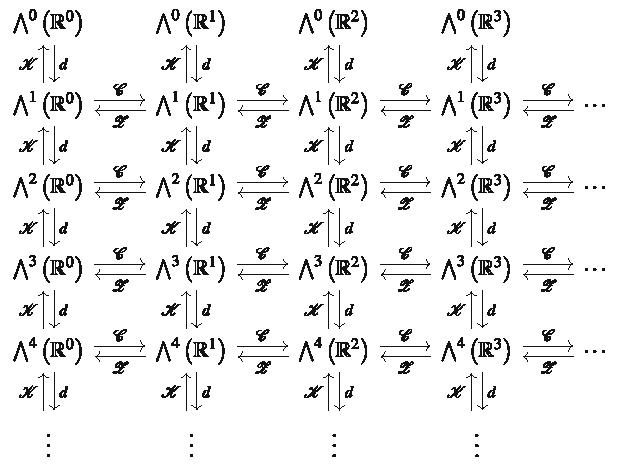
\includegraphics[width=0.856\linewidth]{images/vector/fig-8-5.pdf}
  \caption{有助于理解 Poincaré 引理证明的交换图}
  \label{fig:8-5}
\end{figure}

\begin{figure}[htbp]
  \centering
  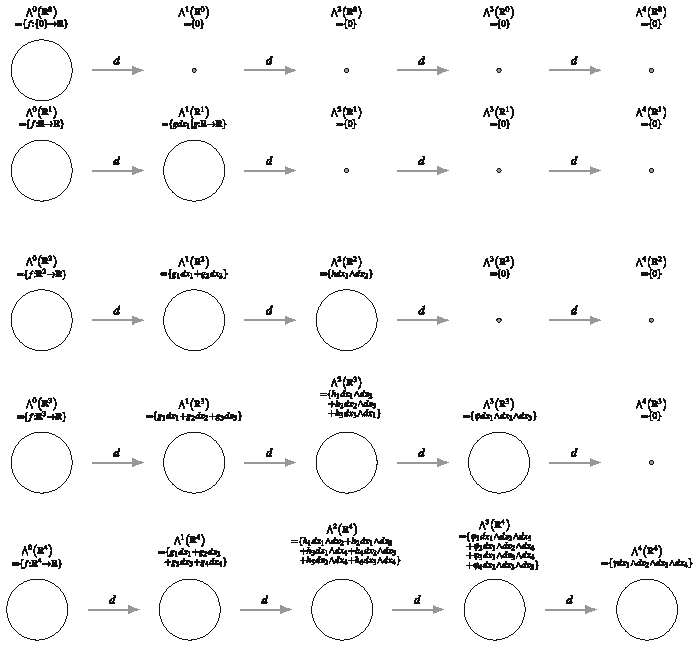
\includegraphics[width=0.960\linewidth]{images/vector/fig-8-6.pdf}
  \caption{这里把图 \ref{fig:8-5} 的列用维恩图式画成行. 归纳假设的基础情形是图 \ref{fig:8-5} 的第一列，此处画成最上一行. 图 \ref{fig:8-5} 的交换图中与我们的中等难度例子相关联的那一列画成第四行}
  \label{fig:8-6}
\end{figure}

\section{基础情形与一个简单例子}

首先我们回忆，$\mathbb{R}^n$ 上的零形式 $\alpha$ 正是 $\mathbb{R}^n$ 上的实值函数. $\mathbb{R}^n$ 上的零形式记为 $\Omega^0(\mathbb{R}^n)$，即图 \ref{fig:8-5} 的最上一行. 虽然 $\mathbb{R}^n$ 上当然可能有闭的零形式，但 $\mathbb{R}^n$ 上不可能有恰当的零形式，因为不存在 $(-1)$-形式这种东西. 因此 Poincaré 引理不适用于零形式，只适用于 $k>0$ 的 $k$-形式.

接下来我们证明基础情形. 每个归纳证明都要求你先证明一个基础情形. 通常——这里也是如此——基础情形非常容易证明. 这正是归纳证明的美妙之处. 这里我们的基础情形是图 \ref{fig:8-5} 的第一列，图 \ref{fig:8-6} 也用维恩图把它画成第一行. $\mathbb{R}^0$ 是恰好含一个点的集合，即 $\mathbb{R}^0=\{0\}$，所以空间 $\Omega^0(\mathbb{R}^0)$ 就是点上的实值函数的集合，即 $f:\{0\}\to\mathbb{R}$. 这在图 \ref{fig:8-5} 的左上角显示为第一个空间.

我们之前还看到过 $\Omega^k(\mathbb{R}^n)=\{0\}$（$k>n$）；也就是说，$\mathbb{R}^n$ 上所有满足 $k>n$ 的 $k$-形式都是零 $k$-形式. 我们的意思是：零 $k$-形式把任意一组 $k$ 个向量都送到零. 因此，对 $k>n$，若 $\alpha\in\Omega^k(\mathbb{R}^n)$，则对每一组向量 $v_1,\ldots,v_k$ 都有 $\alpha(v_1,\ldots,v_k)=0$，因而我们记 $\alpha\equiv0$. 于是对 $k>0$ 有 $\Omega^k(\mathbb{R}^0)=\{0\}$. 这些空间在图 \ref{fig:8-6} 中都画成单点.

现在我们着手证明基础情形. 基础情形的证明本质上很平凡，但仍然分两个简单的步骤：
\begin{enumerate}
  \item 若 $\alpha\in\Omega^1(\mathbb{R}^0)$ 是闭的，证明它是恰当的.
  \item 若 $k>1$ 且 $\alpha\in\Omega^k(\mathbb{R}^0)$ 是闭的，证明它是恰当的.
\end{enumerate}

第一种情形，若 $\alpha\in\Omega^1(\mathbb{R}^0)$，则必有 $\alpha=0$，因为 $\Omega^1(\mathbb{R}^0)$ 中唯一的形式就是零 1-形式. 显然 $d\alpha=d0=0$，所以它是闭的. 为证明它是恰当的，我们必须证明对某个零形式 $f$ 有 $\alpha=df$. 但考虑任意函数 $f\in\Omega^0(\mathbb{R}^0)$. 由于 $f:\{0\}\to\mathbb{R}$，$f(0)$ 就是一个不变的实数. $f$ 的外微分求的是 $f$ 沿任意方向移动时如何变化. 但这里没有可以移动的方向，也不可能发生任何变化，所以对每个 $f\in\Omega^0(\mathbb{R}^0)$ 都必有 $df=0=\alpha$. 因此闭的 $\alpha$ 也是恰当的，第一种情形得证.

第二种情形甚至更容易. 显然，对 $k>1$ 的 $\alpha\in\Omega^k(\mathbb{R}^0)$，由于 $d\alpha=d0=0$，它是闭的. 但 $\alpha$ 是恰当的这一点也是显然的，因为若 $\beta\in\Omega^{k-1}(\mathbb{R}^0)$，则 $d\beta=d0=0=\alpha$. 这样我们也证明了 $\Omega^k(\mathbb{R}^0)$（$k>1$）中任何闭形式都是恰当的. 综合起来，$\mathbb{R}^0$ 上任何闭形式都是恰当的，基础情形得证.

现在，我们不直接进入一般情形，而是用本节剩余部分做一个有点中等难度的例子. 我们这样做是为了帮助你熟悉一般情形中将使用的策略. 一般情形的记号很繁琐，所以在记号不那么铺天盖地时更容易理解基本策略. 我们将证明 $\mathbb{R}^3$ 上的闭 1-形式是恰当的. 图 \ref{fig:8-6} 的第四行展示了图 \ref{fig:8-5} 中与 $\mathbb{R}^3$ 相关联的那部分交换图. 为了做我们的例子，我们需要引入几个映射. 在例子之后、做一般情形之前，我们还要对这些映射多说几句. 第一个映射记为 $Z$，第二个映射记为 $C$；
\[
Z:\Omega^k(\mathbb{R}^n)\to\Omega^k(\mathbb{R}^{n-1}),\qquad
C:\Omega^k(\mathbb{R}^n)\to\Omega^k(\mathbb{R}^{n+1}).
\]
本质上，映射 $Z$ 把 $\mathbb{R}^n$ 上的 $k$-形式``挤压''成 $\mathbb{R}^{n-1}$ 上的 $k$-形式，而映射 $C$ 把 $\mathbb{R}^n$ 上的 $k$-形式``扩张''成 $\mathbb{R}^{n+1}$ 上的 $k$-形式.

假设 $\mathbb{R}^n$ 的坐标函数是 $x_1,\ldots,x_n$. 和往常一样，我们当然有些不严谨，将用同一记号 $x_1,\ldots,x_n$ 既表示 $\mathbb{R}^n$ 上的实值坐标函数，也表示这些函数给出的数值，后者表示点. 也就是说，若 $p\in\mathbb{R}^n$ 且 $x_i$ 是坐标函数 $x_i:\mathbb{R}^n\to\mathbb{R}$，则 $x_i(p)=x_i$，其中左边的 $x_i$ 是坐标函数，右边的 $x_i$ 是数值. 这使我们能够把点写成 $p=(x_1,\ldots,x_n)$. 我们在整个过程中将继续保留这种歧义，并希望它不会给你带来太多困惑.

$\mathbb{R}^n$ 上在点 $p=(x_1,\ldots,x_n)$ 处的零形式就是函数 $f(p)=f(x_1,\ldots,x_n)$；$\mathbb{R}^n$ 上在点 $p$ 处的 1-形式 $\alpha$ 写成 $\alpha=\sum_{i=1}^{n}\alpha_i(p)dx_i=\sum_{i=1}^{n}\alpha_i(x_1,\ldots,x_n)dx_i$；在点 $p$ 处的 2-形式可以写成 $\beta=\sum_{i<j}\beta_{ij}(p)dx_i\wedge dx_j=\sum_{i<j}\beta_{ij}(x_1,\ldots,x_n)dx_i\wedge dx_j$，依此类推. 映射 $Z:\Omega^k(\mathbb{R}^n)\to\Omega^k(\mathbb{R}^{n-1})$ 本质上把 $k$-形式限制到 $\mathbb{R}^n$ 的子空间 $\mathbb{R}^{n-1}$ 上，见图 \ref{fig:8-7}. 它通过把 $x_n$ 的值替换为 0 并消去每个含 $dx_n$ 的项来实现这一点. 于是我们有
\begin{align*}
f(x_1,\ldots,x_{n-1},x_n)\xrightarrow{\;Z\;}f(x_1,\ldots,x_{n-1},0), \\
\sum_{i=1}^{n}\alpha_i(x_1,\ldots,x_{n-1},x_n)dx_i\xrightarrow{\;Z\;}
\sum_{i=1}^{n-1}\alpha_i(x_1,\ldots,x_{n-1},0)dx_i, \\
\sum_{i<j}\beta_{ij}(x_1,\ldots,x_{n-1},x_n)dx_i\wedge dx_j\xrightarrow{\;Z\;}
\sum_{\substack{i<j\\j\neq n}}\beta_{ij}(x_1,\ldots,x_{n-1},0)dx_i\wedge dx_j,
\end{align*}
对 $k>2$ 的 $k$-形式依此类推.

\begin{figure}[htbp]
  \centering
  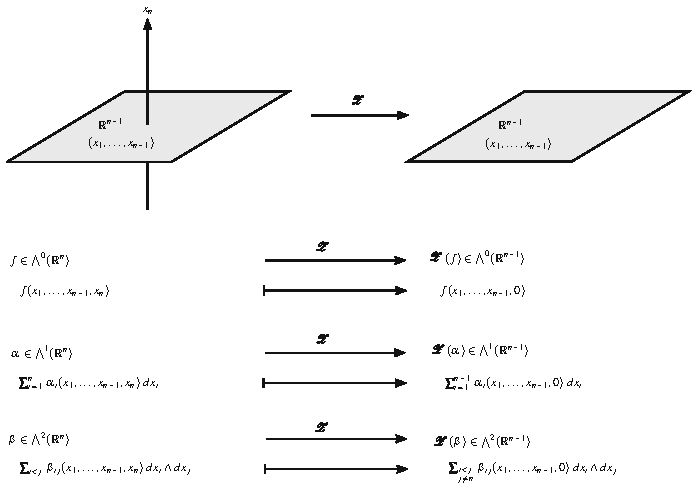
\includegraphics[width=0.960\linewidth]{images/vector/fig-8-7.pdf}
  \caption{映射 $Z:\Omega^k(\mathbb{R}^n)\to\Omega^k(\mathbb{R}^{n-1})$ 的图解. 该映射把 $\mathbb{R}^n$ 上的 $k$-形式``挤压''成 $\mathbb{R}^{n-1}$ 上的 $k$-形式. 这里对零形式、1-形式和 2-形式具体地展示了这一点. $Z$ 令 $x_n=0$ 并消去所有含有 $dx_n$ 的项}
  \label{fig:8-7}
\end{figure}

映射 $C$ 把 $\mathbb{R}^n$ 上的 $k$-形式``扩张''成 $\mathbb{R}^{n+1}$ 上的 $k$-形式，
\begin{align*}
f(x_1,\ldots,x_{n-1},x_n)\xrightarrow{\;C\;}f(x_1,\ldots,x_{n-1},x_n), \\
\sum_{i=1}^{n}\alpha_i(x_1,\ldots,x_{n-1},x_n)dx_i\xrightarrow{\;C\;}
\sum_{i=1}^{n}\alpha_i(x_1,\ldots,x_{n-1},x_n)dx_i, \\
\sum_{i<j}\beta_{ij}(x_1,\ldots,x_{n-1},x_n)dx_i\wedge dx_j\xrightarrow{\;C\;}
\sum_{i<j}\beta_{ij}(x_1,\ldots,x_{n-1},x_n)dx_i\wedge dx_j.
\end{align*}
见图 \ref{fig:8-8}.

\begin{figure}[htbp]
  \centering
  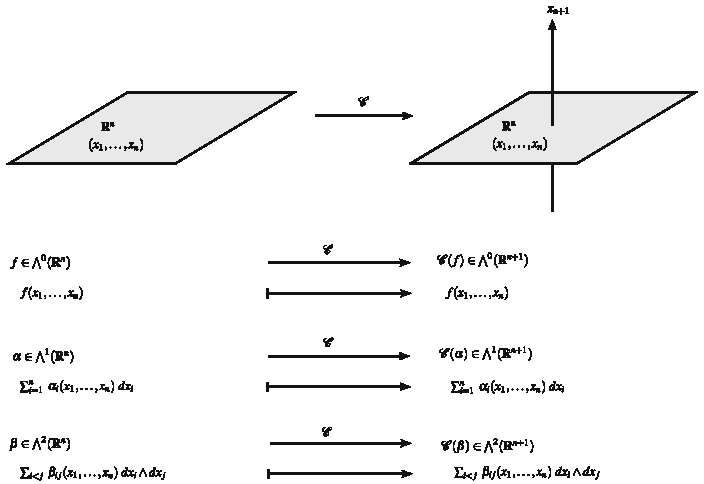
\includegraphics[width=0.960\linewidth]{images/vector/fig-8-8.pdf}
  \caption{映射 $C:\Omega^k(\mathbb{R}^n)\to\Omega^k(\mathbb{R}^{n+1})$ 的图解. 该映射把 $\mathbb{R}^n$ 上的 $k$-形式``扩张''成 $\mathbb{R}^{n+1}$ 上的 $k$-形式. 扩张后的 $\mathbb{R}^{n+1}$ 上的 $k$-形式看起来与 $\mathbb{R}^n$ 上的 $k$-形式完全一样. 这里对零形式、1-形式和 2-形式具体地展示了这一点}
  \label{fig:8-8}
\end{figure}

注意，$f\in\Omega^0(\mathbb{R}^n)$ 看起来与 $C(f)\in\Omega^0(\mathbb{R}^{n+1})$ 完全一样，后者就是一个不依赖于变量 $x_{n+1}$ 的函数. 类似地，$\alpha\in\Omega^1(\mathbb{R}^n)$ 看起来与 $C(\alpha)\in\Omega^1(\mathbb{R}^{n+1})$ 完全一样，后者是 $\mathbb{R}^{n+1}$ 上不含 $dx_{n+1}$ 项、且其分量函数 $\alpha_i$ 完全不依赖于变量 $x_{n+1}$ 的 1-形式. 对 2-形式 $\beta\in\Omega^2(\mathbb{R}^n)$ 也是如此. $C(\beta)$ 看起来与 $\beta$ 完全一样；它是 $\mathbb{R}^{n+1}$ 上不含任何涉及 $dx_{n+1}$ 的项、且其分量函数 $\beta_{ij}$ 不依赖于变量 $x_{n+1}$ 的 2-形式.

为了更好地看清楚这一点，考虑 1-形式 $\alpha=P(x,y,z)dx+Q(x,y,z)dy+R(x,y,z)dz\in\Omega^1(\mathbb{R}^3)$. 那么
\[
Z(\alpha)=P(x,y,0)dx+Q(x,y,0)dy\in\Omega^1(\mathbb{R}^2).
\]
注意我们消掉了含 $dz$ 的项，即 $R(x,y,z)dz$. 现在考虑 1-形式 $\alpha=P(x,y)dx+Q(x,y)dy\in\Omega^1(\mathbb{R}^2)$，那么
\[
C(\alpha)=P(x,y)dx+Q(x,y)dy\in\Omega^1(\mathbb{R}^3).
\]
这个 $\mathbb{R}^3$ 上的 1-形式看起来与 $\mathbb{R}^2$ 上的 1-形式完全一样，尽管它实际上是在 $\mathbb{R}^3$ 上. 它是 $\mathbb{R}^3$ 上不含 $dz$ 项、且分量函数不依赖于变量 $z$ 的 1-形式.

\begin{question}\label{q:8-1}
利用 $\alpha=P(x,y,z)dx+Q(x,y,z)dy+R(x,y,z)dz\in\Omega^1(\mathbb{R}^3)$，证明 $d(Z(\alpha))=Z(d(\alpha))$. 我们常把它写成 $dZ=Zd$.
\end{question}

\begin{question}\label{q:8-2}
利用 $\alpha=P(x,y)dx+Q(x,y)dy\in\Omega^1(\mathbb{R}^2)$，证明 $d(C(\alpha))=C(d(\alpha))$. 我们常把它写成 $dC=Cd$.
\end{question}

\begin{question}\label{q:8-3}
利用 $\alpha=P(x,y,z)dx+Q(x,y,z)dy+R(x,y,z)dz\in\Omega^1(\mathbb{R}^3)$，求 $Z(\alpha)$，然后求 $C(Z(\alpha))$.
\end{question}

除了 $Z$ 和 $C$，我们还需要定义另一个映射 $K:\Omega^1(\mathbb{R}^3)\to\Omega^0(\mathbb{R}^3)$. 若 $\alpha=P(x,y,z)dx+Q(x,y,z)dy+R(x,y,z)dz$ 是 $\mathbb{R}^3$ 上的 1-形式，则 $K(\alpha)$ 是一个零形式，即 $\mathbb{R}^3$ 上的函数，定义为
\[
K(\alpha)=K\left(P(x,y,z)dx+Q(x,y,z)dy+R(x,y,z)dz\right)=\int_0^z R(x,y,t)\,dt.
\]
换言之，$K(\alpha):\mathbb{R}^3\to\mathbb{R}$. 这实际上是如何运作的呢？若给定了 $\mathbb{R}^3$ 上的点 $p=(x_0,y_0,z_0)$，则
\[
K(\alpha)(p)=K(\alpha)(x_0,y_0,z_0)=\int_0^{z_0}R(x_0,y_0,t)\,dt\in\mathbb{R}.
\]

由于 Poincaré 引理讲的是证明闭形式是恰当的，在我们的证明中需要用到一些与闭形式相关的事实. 在这个中等难度的例子中，我们处理的是 $\mathbb{R}^3$ 上的闭 1-形式 $\alpha$. 我们将利用 $d\alpha=0$ 这一事实来找出证明过程中需要的一些恒等式.
\[
\begin{aligned}
d\alpha &= d\left(P(x,y,z)dx+Q(x,y,z)dy+R(x,y,z)dz\right)\\
&= dP\wedge dx+dQ\wedge dy+dR\wedge dz\\
&= \frac{\partial P}{\partial y}dy\wedge dx+\frac{\partial P}{\partial z}dz\wedge dx
  +\frac{\partial Q}{\partial x}dx\wedge dy+\frac{\partial Q}{\partial z}dz\wedge dy
  +\frac{\partial R}{\partial x}dx\wedge dz+\frac{\partial R}{\partial y}dy\wedge dz\\
&= \left(\frac{\partial Q}{\partial x}-\frac{\partial P}{\partial y}\right)dx\wedge dy
  +\left(\frac{\partial R}{\partial x}-\frac{\partial P}{\partial z}\right)dx\wedge dz
  +\left(\frac{\partial R}{\partial y}-\frac{\partial Q}{\partial z}\right)dy\wedge dz\\
&= 0
\end{aligned}
\]
因此这个 2-形式的每一项的系数都等于零，从而给出下面三个恒等式
\[
\frac{\partial Q}{\partial x}=\frac{\partial P}{\partial y},\qquad
\frac{\partial R}{\partial x}=\frac{\partial P}{\partial z},\qquad
\frac{\partial R}{\partial y}=\frac{\partial Q}{\partial z}.
\]

既然所有必要的准备终于落实了，我们就准备好在我们这个例子中证明 Poincaré 引理了. 我们首先给出总体策略. 之后我们给出每一步的细节. 假设我们知道 $\alpha\in\Omega^1(\mathbb{R}^3)$ 是闭的. 我们的目标是证明 $\alpha$ 也是恰当的. 也就是说，我们想证明存在某个 $\beta\in\Omega^0(\mathbb{R}^3)$ 使得 $d\beta=\alpha$. 首先我们给出我们想做什么的一般思路，图 \ref{fig:8-9} 给出了示意. 我们先用 $Z$ 把 $\alpha$``挤压''下来得到 $Z(\alpha)\in\Omega^1(\mathbb{R}^2)$，由归纳假设可以证明它是恰当的. 然后用 $C$ 把恰当形式 $Z(\alpha)$``扩张''得到 $C(Z(\alpha))\in\Omega^1(\mathbb{R}^3)$，它也可以被证明是恰当的. 由于 $C(Z(\alpha))$ 在某种意义上只是 $\alpha$ 的一部分，我们想证明 $\alpha$ 的其余部分，即 $\alpha-C(Z(\alpha))$，也是恰当的. 我们可以通过对 $\alpha$ 使用 $K$ 得到 $K(\alpha)\in\Omega^0(\mathbb{R}^3)$，然后取它的外微分得到 $d(K(\alpha))\in\Omega^1(\mathbb{R}^3)$，后者显然是恰当的. 事实证明
\[
\underbrace{d(K(\alpha))}_{\text{由定义显然恰当}}=\alpha-\underbrace{C(Z(\alpha))}_{\text{由归纳假设恰当}}.
\]
换言之，我们有
\[
d(K(\alpha))=\alpha-C(Z(\alpha)).
\]
但这就意味着
\[
\begin{aligned}
\alpha &= \underbrace{C(Z(\alpha))}_{\substack{\text{恰当，故存在某个 }\omega\\\text{使得 }C(Z(\alpha))=d\omega}}+\underbrace{d(K(\alpha))}_{\text{由定义显然恰当}}\\
&= d\omega+d(K(\alpha))\\
&= d\left(\omega+K(\alpha)\right)\qquad\text{（由 }d\text{ 的线性）}
\end{aligned}
\]
因此 $\alpha$ 本身是恰当的，这正是我们要证明的. 注意我们从未显式给出 $\omega$ 是什么. 换言之，虽然我们在逻辑上推理出 $\omega$ 必定存在，但我们从未真正找到 $\omega$ 的显式公式.

\begin{figure}[htbp]
  \centering
  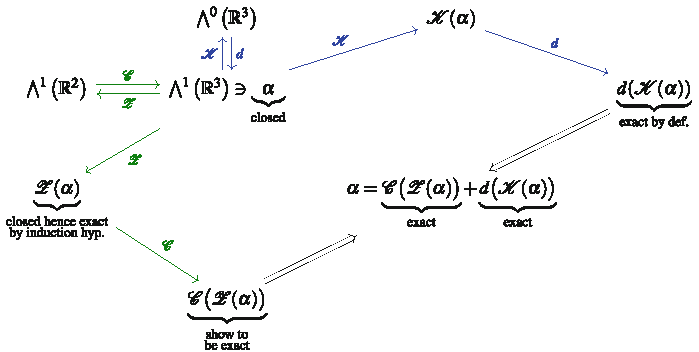
\includegraphics[width=0.960\linewidth]{images/vector/fig-8-9.pdf}
  \caption{我们例子证明的一般思路. 对 $\alpha\in\Omega^1(\mathbb{R}^3)$，我们计算 $K(\alpha)\in\Omega^0(\mathbb{R}^3)$，然后计算 $d(K(\alpha))\in\Omega^1(\mathbb{R}^3)$，后者显然是恰当的. 我们还计算 $Z(\alpha)\in\Omega^1(\mathbb{R}^2)$，它是闭的，因而由归纳假设是恰当的. 然后计算 $C(Z(\alpha))\in\Omega^1(\mathbb{R}^3)$，可以证明它也是恰当的. 于是可以证明 $\alpha=C(Z(\alpha))+d(K(\alpha))$，即两个恰当项之和，这意味着 $\alpha$ 本身是恰当的}
  \label{fig:8-9}
\end{figure}

现在我们已经把将要采用的总体策略告诉了你，就可以着手细节了. 我们现在需要证明两件事：第一，$C(Z(\alpha))$ 由归纳假设是恰当的；第二，$d(K(\alpha))=\alpha-C(Z(\alpha))$. 证明这两件事实际上正是整个证明的精华. 由于 $\alpha$ 是闭的，由闭的定义有 $d\alpha=0$. 利用 $dZ=Zd$ 这一事实，我们有
\[
d(Z(\alpha))=Z(d\alpha)=Z(0)=0\qquad\Rightarrow\qquad Z(\alpha)\in\Omega^1(\mathbb{R}^2)\ \text{是闭的}.
\]
归纳假设是说 $\mathbb{R}^2$ 上所有闭 1-形式都已知是恰当的. 由于 $Z(\alpha)$ 是 $\mathbb{R}^2$ 上已知是闭的 1-形式，由归纳假设我们知道 $Z(\alpha)$ 是恰当的. 这意味着 $\mathbb{R}^2$ 上存在某个零形式 $\omega$ 使得 $Z(\alpha)=d\omega$. 为了证明 $C(Z(\alpha))\in\Omega^1(\mathbb{R}^3)$ 是恰当的，我们利用 $dC=Cd$ 这一事实，
\[
C(Z(\alpha))=C(d\omega)=d(C\omega)\qquad\Rightarrow\qquad C(Z(\alpha))\in\Omega^1(\mathbb{R}^3)\ \text{是恰当的}.
\]
现在我们将证明 $d(K(\alpha))$ 是 $\alpha$ 减去恰当部分 $C(Z(\alpha))$ 后剩下的部分；也就是说，$d(K(\alpha))=\alpha-C(Z(\alpha))$. 这通过一个显式计算完成：
\[
\begin{aligned}
d(K(\alpha)) &= d\left(K\left(P(x,y,z)dx+Q(x,y,z)dy+R(x,y,z)dz\right)\right)\\
&= d\left(\int_0^z R(x,y,t)\,dt\right)\\
&= \frac{\partial}{\partial x}\left(\int_0^z R(x,y,t)\,dt\right)dx\\
&\qquad+\frac{\partial}{\partial y}\left(\int_0^z R(x,y,t)\,dt\right)dy\\
&\qquad+\frac{\partial}{\partial z}\left(\int_0^z R(x,y,t)\,dt\right)dz\\
&= \left(\int_0^z\frac{\partial R(x,y,t)}{\partial x}\,dt\right)dx\\
&\qquad+\left(\int_0^z\frac{\partial R(x,y,t)}{\partial y}\,dt\right)dy+R(x,y,z)\,dz\\
&\quad\text{（对 }x\text{、}y\text{ 的偏导可直接移入积分号内；最后一项由微积分基本定理）}\\
&= \left(\int_0^z\frac{\partial P(x,y,t)}{\partial t}\,dt\right)dx\\
&\qquad+\left(\int_0^z\frac{\partial Q(x,y,t)}{\partial t}\,dt\right)dy+R(x,y,z)\,dz\\
&\quad\text{（}\alpha\text{ 闭 }\Rightarrow\tfrac{\partial R}{\partial x}=\tfrac{\partial P}{\partial z}\text{，}\alpha\text{ 闭 }\Rightarrow\tfrac{\partial R}{\partial y}=\tfrac{\partial Q}{\partial z}\text{）}\\
&= \left(P(x,y,z)-P(x,y,0)\right)dx+\left(Q(x,y,z)-Q(x,y,0)\right)dy+R(x,y,z)\,dz\\
&= \left(P(x,y,z)dx+Q(x,y,z)dy+R(x,y,z)dz\right)-\left(P(x,y,0)dx+Q(x,y,0)dy\right)\\
&= \alpha-C(Z(\alpha))
\end{aligned}
\]
于是
\begin{align*}
d(K(\alpha))=\alpha-C(Z(\alpha)) \\
\Rightarrow\quad \alpha=d(K(\alpha))+C(Z(\alpha)),
\end{align*}
其中 $\underbrace{d(K(\alpha))\ \text{由定义恰当}}_{}$，$\underbrace{C(Z(\alpha))\ \text{由上面恰当}}_{}$.
\[
\Rightarrow\qquad \alpha\ \text{是恰当的}.
\]
这样我们就在我们的例子中证明了 Poincaré 引理. 我们证明了若 $\alpha\in\Omega^1(\mathbb{R}^3)$ 是闭的，则 $\alpha$ 也是恰当的.

现在有几条评注. 在 Poincaré 引理的一般证明中，我们将证明若 $\alpha$ 是 $\mathbb{R}^n$ 上的闭 $k$-形式，则它是恰当的. 我们的证明要求我们假设所谓的归纳假设. 在这里，为了证明 $\mathbb{R}^n$ 上的闭 $k$-形式是恰当的，我们利用 $\mathbb{R}^{n-1}$ 上的闭 $k$-形式是恰当的这一事实. 由我们的基础情形，我们已经证明了 $\mathbb{R}^0$ 上任何闭 $k$-形式都是恰当的.

一般证明对任意 $n$ 成立，所以若取 $n=1$，我们就能证明 $\mathbb{R}^1$ 上任何闭 $k$-形式都是恰当的. 我们在 Poincaré 引理的一般证明中证明这一点，这要求我们使用归纳假设. 在 $n=1$ 的情形中，我们的归纳假设是 $\mathbb{R}^0$ 上任何闭 $k$-形式都是恰当的，这我们已经知道了. 然后，一旦我们知道这一点，就可以用它来证明 $\mathbb{R}^1$ 上闭 $k$-形式是恰当的. 一旦这已知，同样的论证可以用来证明 $\mathbb{R}^2$ 上闭 $k$-形式是恰当的，这又可以用来证明 $\mathbb{R}^3$ 上闭 $k$-形式是恰当的，这又可以用来……如此等等. 这样我们就可以自举而上，证明我们想要的任何 $\mathbb{R}^n$ 上闭 $k$-形式都是恰当的.

当然，我们不想把同样的论证一遍又一遍地重复无穷多次，所以我们只做一次，但做的方式要足够一般，使之对我们想要的任何 $k$ 和 $n$ 的值都成立. 这意味着我们的记号必须非常一般，这可能会让我们的论证在记号上有点压得人喘不过气. 这就是我们为什么先做一个简单例子的原因之一，这样你可以在不被试图跟上所有记号分心的情况下感受论证的运作方式. 我们还要说明，如果我们对例子中所做的稍作改动，一般证明会更容易. 等时机成熟时我们会解释这一点.

\section{一般情形}

在 Poincaré 引理证明的一般情形中，我们将证明对任意的 $k$ 和 $n$，$\mathbb{R}^{n+1}$ 上的闭 $k$-形式都是恰当的. 但在投入一般情形的证明之前，让我们重新审视一下 $Z$ 和 $C$ 这两个映射，确保我们理解它们是什么，以及它们对任意 $k$ 和 $n$ 如何运作. 事实证明，$Z$ 和 $C$ 是两个简单映射的\newterm{pull-back}{拉回}{pull-back}. 我们先考察 $Z$.

考虑图 \ref{fig:8-10} 所示的记为 $S$ 的拉伸映射，
\[
S:\mathbb{R}^n\to\mathbb{R}^{n+1},\qquad (x_1,\ldots,x_n)\longmapsto(x_1,\ldots,x_n,0).
\]
注意这里有些歧义. 除了把 $x_i$ 既用作坐标函数的记号又用作数值之外，我们还把 $x_i$ 用作 $\mathbb{R}^n$ 和 $\mathbb{R}^{n+1}$ 两个空间的坐标函数. 我们想稍微小心一点，在头脑中把空间区分开来，所以我们说 $x_1,\ldots,x_n$ 是 $\mathbb{R}^n$ 上的坐标函数，$y_1,\ldots,y_{n+1}$ 是 $\mathbb{R}^{n+1}$ 上的坐标函数. 严格地说我们会写
\[
S:\mathbb{R}^n\to\mathbb{R}^{n+1},\qquad
(x_1,\ldots,x_n)\longmapsto\left(y_1(x_1,\ldots,x_n),\ldots,y_{n+1}(x_1,\ldots,x_n)\right),
\]
其中
\[
y_1(x_1,\ldots,x_n)=x_1,\quad\ldots\quad
y_n(x_1,\ldots,x_n)=x_n,\quad
y_{n+1}(x_1,\ldots,x_n)=0.
\]
当然，映射 $S$ 给出 $k$-形式的拉回映射 $T^*S\equiv S^*$，
\[
\Omega^k(\mathbb{R}^{n+1})\xleftarrow{\;T^*S\;}\Omega^k(\mathbb{R}^n),\qquad
S:\mathbb{R}^n\to\mathbb{R}^{n+1}.
\]
这显示在图 \ref{fig:8-11} 中.

\begin{figure}[htbp]
  \centering
  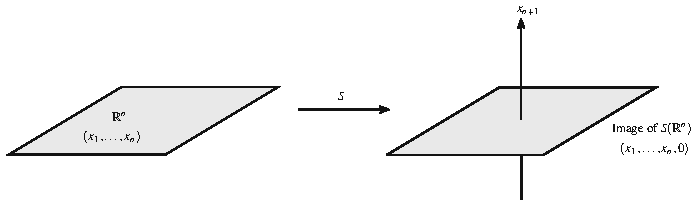
\includegraphics[width=0.960\linewidth]{images/vector/fig-8-10.pdf}
  \caption{映射 $S:\mathbb{R}^n\to\mathbb{R}^{n+1}$}
  \label{fig:8-10}
\end{figure}

$\mathbb{R}^{n+1}$ 上 $k$-形式的基本构件具有形式 $f_{i_1\cdots i_k}dy_{i_1}\wedge dy_{i_2}\wedge\cdots\wedge dy_{i_k}$，其中按约定有 $i_1<i_2<\cdots<i_k\leq n+1$. 利用第 6.7 节中第二和第三个恒等式，并利用零形式的拉回（也在第 6.7 节讲过），我们计算这些 $k$-形式基本构件之一的拉回，
\[
\begin{aligned}
&T^*S\cdot\left(f_{i_1\cdots i_k}dy_{i_1}\wedge dy_{i_2}\wedge\cdots\wedge dy_{i_k}\right)\\
&= T^*Sf_{i_1\cdots i_k}\cdot T^*Sdy_{i_1}\wedge T^*Sdy_{i_2}\wedge\cdots\wedge T^*Sdy_{i_k}\\
&= (f_{i_1\cdots i_k}\circ S)\cdot d(S^*y_{i_1})\wedge d(S^*y_{i_2})\wedge\cdots\wedge d(S^*y_{i_k})\\
&= (f_{i_1\cdots i_k}\circ S)\cdot d(y_{i_1}\circ S)\wedge d(y_{i_2}\circ S)\wedge\cdots\wedge d(y_{i_k}\circ S)\\
&= (f_{i_1\cdots i_k}\circ S)\cdot\left(\sum_{j=1}^{n}\frac{\partial y_{i_1}(x_1,\ldots,x_n)}{\partial x_j}dx_j\right)
  \wedge\cdots\wedge\left(\sum_{j=1}^{n}\frac{\partial y_{i_k}(x_1,\ldots,x_n)}{\partial x_j}dx_j\right)\\
&=\begin{cases}
f_{i_1\cdots i_k}(x_1,\ldots,x_n,0)\,dx_{i_1}\wedge\cdots\wedge dx_{i_k}, & \text{若 } i_k\neq n+1,\\
0, & \text{若某个 } i=n+1.
\end{cases}
\end{aligned}
\]
最后一个等式由 $y_i(x_1,\ldots,x_n)$ 的定义得出. 对每个满足 $1\leq i_l\leq n+1$ 的 $i_l$，我们有
\[
\sum_{j=1}^{n}\frac{\partial y_i(x_1,\ldots,x_n)}{\partial x_j}dx_j=
\begin{cases}
\displaystyle\sum_{j=1}^{n}\frac{\partial x_i}{\partial x_j}dx_j=dx_i, & \text{若 } i\neq n+1,\\
\displaystyle\sum_{j=1}^{n}\frac{\partial 0}{\partial x_j}dx_j=0, & \text{若 } i=n+1.
\end{cases}
\]
这正是我们之前的映射 $Z$，因此 $Z=T^*S$. 用这个公式以及拉回的线性（即第 6.7 节的第一个恒等式），可以拉回完整的 $k$-形式. 换言之，只需把这个公式应用于 $k$-形式的每一项即可.

\begin{figure}[htbp]
  \centering
  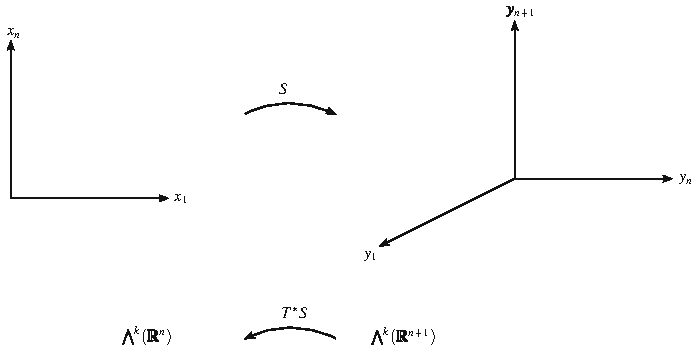
\includegraphics[width=0.960\linewidth]{images/vector/fig-8-11.pdf}
  \caption{用更合适的坐标函数记号表示的映射 $S:\mathbb{R}^n\to\mathbb{R}^{n+1}$，以及拉回映射 $T^*S\equiv S^*:\Omega^k(\mathbb{R}^{n+1})\to\Omega^k(\mathbb{R}^n)$}
  \label{fig:8-11}
\end{figure}

\begin{question}\label{q:8-4}
对 $S:\mathbb{R}^2\to\mathbb{R}^3$ 和 $\alpha=P(x,y,z)dx+Q(x,y,z)dy+R(x,y,z)dz\in\Omega^1(\mathbb{R}^3)$，证明上面定义的 $T^*S\cdot\alpha$ 与 $Z(\alpha)$ 相同.
\end{question}

现在我们转向 $C$. 现在我们考虑另一个不同的映射——投影映射，记为 $P$，如图 \ref{fig:8-12} 所示，
\[
P:\mathbb{R}^{n+1}\to\mathbb{R}^n,\qquad
(y_1,\ldots,y_{n+1})\longmapsto\left(x_1(y_1,\ldots,y_{n+1}),\ldots,x_n(y_1,\ldots,y_{n+1})\right),
\]
其中
\[
x_1(y_1,\ldots,y_{n+1})=y_1,\quad\ldots\quad
x_n(y_1,\ldots,y_{n+1})=y_n.
\]
这就给出拉回映射 $T^*P\equiv P^*$，
\[
\Omega^k(\mathbb{R}^{n+1})\xleftarrow{\;T^*P\;}\Omega^k(\mathbb{R}^n),\qquad
P:\mathbb{R}^{n+1}\to\mathbb{R}^n.
\]
$\mathbb{R}^n$ 上 $k$-形式的基本构件是 $f_{i_1\cdots i_k}dx_{i_1}\wedge\cdots\wedge dx_{i_k}$，其中 $i_1<i_2<\cdots<i_k$. 我们计算
\[
\begin{aligned}
&T^*P\cdot\left(f_{i_1\cdots i_k}dx_{i_1}\wedge\cdots\wedge dx_{i_k}\right)\\
&= (T^*Pf_{i_1\cdots i_k})\cdot T^*Pdx_{i_1}\wedge\cdots\wedge T^*Pdx_{i_k}\\
&= (f_{i_1\cdots i_k}\circ P)\cdot d(T^*Px_{i_1})\wedge\cdots\wedge d(T^*Px_{i_k})\\
&= (f_{i_1\cdots i_k}\circ P)\cdot d(x_{i_1}\circ P)\wedge\cdots\wedge d(x_{i_k}\circ P)\\
&= f_{i_1\cdots i_k}(y_1,\ldots,y_{n+1})\,dy_{i_1}\wedge\cdots\wedge dy_{i_k}.
\end{aligned}
\]
因此我们看到我们的映射恰好就是 $C=P^*$.

\begin{figure}[htbp]
  \centering
  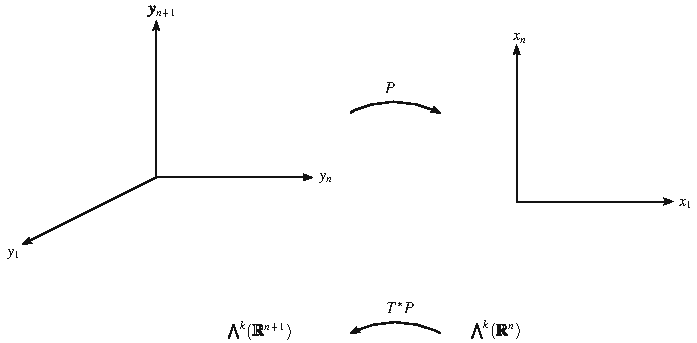
\includegraphics[width=0.960\linewidth]{images/vector/fig-8-12.pdf}
  \caption{映射 $P:\mathbb{R}^{n+1}\to\mathbb{R}^n$ 以及拉回映射 $T^*P\equiv P^*:\Omega^k(\mathbb{R}^n)\to\Omega^k(\mathbb{R}^{n+1})$}
  \label{fig:8-12}
\end{figure}

\begin{question}\label{q:8-5}
证明上面的最后一个等式，也就是说，对 $1\leq l\leq k\leq n$ 证明 $dx_{i_l}=dy_{i_l}$.
\end{question}

\begin{question}\label{q:8-6}
证明对任意 $k$-形式 $\beta$ 有 $Z(C(\beta))=\beta$.
\end{question}

由于 $C=P^*$、$Z=S^*$，并且我们已经从拉回和外微分的性质知道 $dP^*=P^*d$、$dS^*=S^*d$，所以我们自动得到 $dC=Cd$ 和 $dZ=Zd$.

在一般情形中，映射 $K:\Omega^k(\mathbb{R}^{n+1})\to\Omega^{k-1}(\mathbb{R}^{n+1})$ 由下式给出
若 $i_k\neq n+1$，则
\[
K\left(f(x_1,\ldots,x_{n+1})dx_{i_1}\wedge\cdots\wedge dx_{i_k}\right)=0.
\]
若 $i_k=n+1$，则
\[
K\left(f(x_1,\ldots,x_{n+1})dx_{i_1}\wedge\cdots\wedge dx_{i_k}\right)
=\left(\int_0^{x_{n+1}}f(x_1,\ldots,x_n,t)\,dt\right)dx_{i_1}\wedge\cdots\wedge dx_{i_{k-1}}.
\]
映射 $K:\Omega^{k+1}(\mathbb{R}^{n+1})\to\Omega^k(\mathbb{R}^{n+1})$ 是类似的，只是做了相应调整.

我们现在准备证明 Poincaré 引理的一般情形. 假设我们有 $\alpha\in\Omega^k(\mathbb{R}^{n+1})$，它是闭的. 也就是说，$d\alpha=0$. 我们将用到的各种映射显示在图 \ref{fig:8-13} 的上方，我们要做什么的一般示意显示在下方. 在例子中我们证明了 $\alpha=CZ\alpha+d(K\alpha)$. 我们还证明了 $CZ\alpha$ 是恰当的，并且显然 $d(K\alpha)$ 是恰当的，所以可以推出 $\alpha$ 是恰当的. 事实证明，在一般情形中，证明更一般的结论反而更容易：对任意闭 $k$-形式 $\alpha$ 都有
\[
\alpha=CZ\alpha+(-1)^{k-1}\left(d(K\alpha)+Kd\alpha\right)
=\left(CZ+(-1)^{k-1}(dK+Kd)\right)\alpha.
\]
我们为什么要这样做呢？问题在于，一般来说 $\mathbb{R}^{n+1}$ 上的 $k$-形式 $\alpha$ 具有形式
\[
\alpha=\sum\alpha_{j_1\cdots j_k}(x_1,x_2,\ldots,x_{n+1})dx_{j_1}\wedge\cdots\wedge dx_{j_k},
\]
其中每个 $\alpha_{j_1\cdots j_k}$ 都是实值函数，当然还有 $j_1<\cdots<j_k$. 虽然 $\alpha$ 整体可能是闭的，但和式中的每一项未必是闭的，事实上很可能不是闭的. 这正是问题所在. 为简单起见，我们希望证明中的计算一次只对和式中的一项进行. 也就是说，我们希望分别对和式中的每一项 $\alpha_{j_1\cdots j_k}(x_1,x_2,\ldots,x_{n+1})dx_{j_1}\wedge\cdots\wedge dx_{j_k}$ 进行计算. 能够这样做会使计算简单得多. 然后我们可以只用线性把我们的结果应用于整个 $\alpha$，它只是各项之和.

\begin{figure}[htbp]
  \centering
  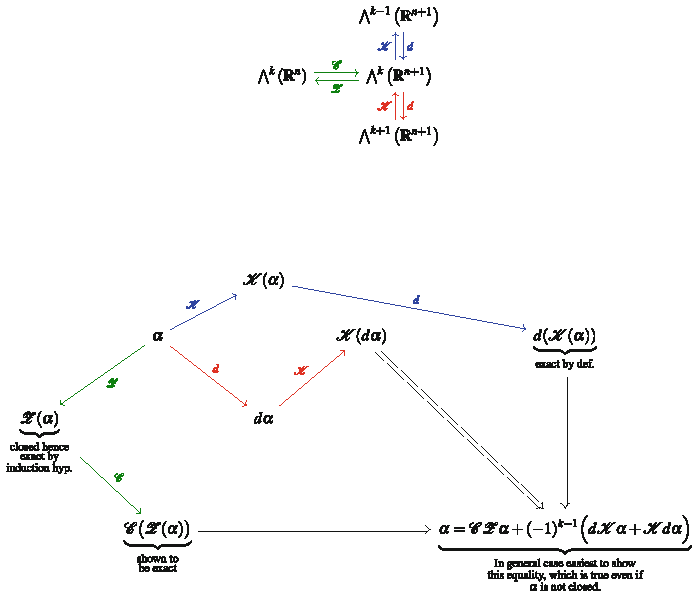
\includegraphics[width=0.960\linewidth]{images/vector/fig-8-13.pdf}
  \caption{Poincaré 引理一般情形证明中重要的各种映射显示在上方，一般情形证明的示意图显示在下方. 回顾 $k$-形式 $\alpha$ 具有形式 $\alpha=\sum\alpha_{i_1\cdots i_k}dx_{i_1}\wedge\cdots\wedge dx_{i_k}$，其中每个 $\alpha_{i_1\cdots i_k}$ 是流形上的函数. 虽然整个 $k$-形式 $\alpha$ 可能是闭的，但组成 $\alpha$ 的每一项 $\alpha_{i_1\cdots i_k}dx_{i_1}\wedge\cdots\wedge dx_{i_k}$ 却未必是闭的. 推导出的公式 $\alpha=CZ\alpha+(-1)^{k-1}(dK\alpha+Kd\alpha)$ 对其中每一项成立. 利用线性，该公式对 $\alpha$ 整体成立；若 $\alpha$ 是闭的，则公式化为 $\alpha=CZ\alpha+(-1)^{k-1}dK\alpha$，后者被证明是恰当的}
  \label{fig:8-13}
\end{figure}

证明的第一部分——证明 $CZ\alpha$ 是恰当的——与之前相同. 由于 $\alpha$ 是闭的，由闭的定义有 $d\alpha=0$，于是
\[
d(C\alpha)=C(d\alpha)=C(0)=0,
\]
所以 $C\alpha$ 也是闭的. 但 $C\alpha\in\Omega^k(\mathbb{R}^n)$，而我们的归纳假设是 $\mathbb{R}^n$ 上所有闭形式都是恰当的. 由归纳假设，由于 $C\alpha$ 是闭的，它也是恰当的，所以对某个 $\beta$ 有 $C\alpha=d\beta$. 于是
\[
ZC\alpha=Zd\beta=dZ\beta.
\]
但这意味着 $ZC\alpha$ 是形式 $Z\beta$ 的外微分，由恰当性的定义，这意味着 $ZC\alpha$ 是恰当的. 这样我们就证明了若 $\alpha$ 是闭的，则 $ZC\alpha$ 是恰当的.

现在我们转向要证明的恒等式. 我们需要把对 $\alpha$ 的一个基本构件元素的证明分成两种情形，一种 $j_k=n+1$，一种 $j_k\neq n+1$.

\textbf{情形一：} $j_k=n+1$

我们考虑单项形式 $f(x_1,\ldots,x_{n+1})dx_{j_1}\wedge\cdots\wedge dx_{j_k}$，其中 $j_1<j_2<\cdots<j_k$ 且 $j_k=n+1$，
\[
\begin{aligned}
&dK\left(f(x_1,\ldots,x_{n+1})dx_{j_1}\wedge\cdots\wedge dx_{j_k}\right)\\
&= d\left(\int_0^{x_{n+1}}f(x_1,\ldots,x_n,t)\,dt\,dx_{j_1}\wedge\cdots\wedge dx_{j_{k-1}}\right)\\
&= \sum_{i=1}^{n+1}\frac{\partial}{\partial x_i}\left(\int_0^{x_{n+1}}f(x_1,\ldots,x_n,t)\,dt\right)dx_i\wedge dx_{j_1}\wedge\cdots\wedge dx_{j_{k-1}}\\
&= \sum_{i=1}^{n}\left(\int_0^{x_{n+1}}\frac{\partial f(x_1,\ldots,x_n,t)}{\partial x_i}\,dt\right)dx_i\wedge dx_{j_1}\wedge\cdots\wedge dx_{j_{k-1}}\\
&\qquad +f(x_1,\ldots,x_{n+1})\,dx_{n+1}\wedge dx_{j_1}\wedge\cdots\wedge dx_{j_{k-1}}.
\end{aligned}
\]
接下来计算
\[
\begin{aligned}
&Kd\left(f(x_1,\ldots,x_{n+1})dx_{j_1}\wedge\cdots\wedge dx_{j_k}\right)\\
&= K\left(\sum_{i=1}^{n+1}\frac{\partial f(x_1,\ldots,x_{n+1})}{\partial x_i}dx_i\wedge dx_{j_1}\wedge\cdots\wedge dx_{j_k}\right)\\
&= \sum_{i=1}^{n}K\left(\frac{\partial f(x_1,\ldots,x_{n+1})}{\partial x_i}dx_i\wedge dx_{j_1}\wedge\cdots\wedge dx_{j_k}\right)\\
&= \sum_{i=1}^{n}\left(\int_0^{x_{n+1}}\frac{\partial f(x_1,\ldots,x_n,t)}{\partial x_i}\,dt\right)dx_i\wedge dx_{j_1}\wedge\cdots\wedge dx_{j_k}.
\end{aligned}
\]
将第一个式子减去第二个式子，并回忆 $j_k=n+1$，再注意到
\[
CZ\left(f(x_1,\ldots,x_{n+1})dx_{j_1}\wedge\cdots\wedge dx_{j_{k-1}}\wedge dx_{n+1}\right)=0,
\]
我们得到
\[
\begin{aligned}
&(dK-Kd)\left(f(x_1,\ldots,x_{n+1})dx_{j_1}\wedge\cdots\wedge dx_{j_k}\right)\\
&= f(x_1,\ldots,x_{n+1})dx_{n+1}\wedge dx_{j_1}\wedge\cdots\wedge dx_{j_{k-1}}\\
&= (-1)^{k-1}f(x_1,\ldots,x_{n+1})dx_{j_1}\wedge\cdots\wedge dx_{j_{k-1}}\wedge dx_{n+1}-0\\
&= (-1)^{k-1}\left(1-CZ\right)\left(f(x_1,\ldots,x_{n+1})dx_{j_1}\wedge\cdots\wedge dx_{j_{k-1}}\wedge dx_{n+1}\right).
\end{aligned}
\]
稍作整理，并记 $\omega=f(x_1,\ldots,x_{n+1})dx_{j_1}\wedge\cdots\wedge dx_{j_k}$（它本身实际上未必是闭的），就得到我们想要的，即
\[
\omega=CZ\omega+(-1)^{k-1}\left(dK\omega-Kd\omega\right).
\]

\begin{question}\label{q:8-7}
证明 $CZ\left(f(x_1,\ldots,x_{n+1})dx_{j_1}\wedge\cdots\wedge dx_{j_{k-1}}\wedge dx_{n+1}\right)=0$.
\end{question}

\textbf{情形二：} $j_k\neq n+1$

我们考虑单项形式 $f(x_1,\ldots,x_{n+1})dx_{j_1}\wedge\cdots\wedge dx_{j_k}$，其中 $j_1<j_2<\cdots<j_k$ 但 $j_k\neq n+1$. 这里，由映射 $K$ 的定义，我们有
\[
dK\left(f(x_1,\ldots,x_{n+1})dx_{j_1}\wedge\cdots\wedge dx_{j_k}\right)=0.
\]
现在我们计算
\[
\begin{aligned}
&Kd\left(f(x_1,\ldots,x_{n+1})dx_{j_1}\wedge\cdots\wedge dx_{j_k}\right)\\
&= K\left(\sum_{i=1}^{n+1}\frac{\partial f(x_1,\ldots,x_{n+1})}{\partial x_i}dx_i\wedge dx_{j_1}\wedge\cdots\wedge dx_{j_k}\right)\\
&= K\Biggl(\sum_{i=1}^{n}\frac{\partial f(x_1,\ldots,x_{n+1})}{\partial x_i}dx_i\wedge dx_{j_1}\wedge\cdots\wedge dx_{j_k}\\
&\quad+\frac{\partial f(x_1,\ldots,x_{n+1})}{\partial x_{n+1}}dx_{n+1}\wedge dx_{j_1}\wedge\cdots\wedge dx_{j_k}\Biggr)\\
&\quad\text{（}K\text{ 消去所有这些不含 }dx_{n+1}\text{ 的项）}\\
&= K\left((-1)^k\frac{\partial f(x_1,\ldots,x_{n+1})}{\partial x_{n+1}}dx_{j_1}\wedge\cdots\wedge dx_{j_k}\wedge dx_{n+1}\right)\\
&= (-1)^k\left(\int_0^{x_{n+1}}\frac{\partial f(x_1,\ldots,x_n,t)}{\partial x_{n+1}}\,dt\right)dx_{j_1}\wedge\cdots\wedge dx_{j_k}\\
&= (-1)^k\left(f(x_1,\ldots,x_n,x_{n+1})-f(x_1,\ldots,x_n,0)\right)dx_{j_1}\wedge\cdots\wedge dx_{j_k}\\
&\quad\text{（微积分基本定理）}
\end{aligned}
\]
将第二个式子从第一个式子中减去，得到
\[
\begin{aligned}
&(dK-Kd)\left(f(x_1,\ldots,x_{n+1})dx_{j_1}\wedge\cdots\wedge dx_{j_k}\right)\\
&= 0-(-1)^k\left(f(x_1,\ldots,x_n,x_{n+1})-f(x_1,\ldots,x_n,0)\right)dx_{j_1}\wedge\cdots\wedge dx_{j_k}\\
&= (-1)^{k-1}\left(f(x_1,\ldots,x_n,x_{n+1})dx_{j_1}\wedge\cdots\wedge dx_{j_k}-f(x_1,\ldots,x_n,0)dx_{j_1}\wedge\cdots\wedge dx_{j_k}\right).
\end{aligned}
\]
但若 $j_k\neq n+1$，则
\[
CZ\left(f(x_1,\ldots,x_{n+1})dx_{j_1}\wedge\cdots\wedge dx_{j_k}\right)=f(x_1,\ldots,x_n,0)dx_{j_1}\wedge\cdots\wedge dx_{j_k},
\]
所以令 $\omega=f(x_1,\ldots,x_{n+1})dx_{j_1}\wedge\cdots\wedge dx_{j_k}$，我们有
\begin{align*}
(dK-Kd)\omega=(-1)^{k-1}\left(\omega-CZ\omega\right) \\
\Rightarrow\qquad \omega=CZ\omega+(-1)^{k-1}\left(dK\omega-Kd\omega\right),
\end{align*}
这与情形一中得到的公式完全相同.

因此，无论 $j_k=n+1$ 还是 $j_k\neq n+1$，对 $k$-形式 $\alpha$ 的每一项 $\omega$ 我们都得到完全相同的恒等式，即
\[
\omega=CZ\omega+(-1)^{k-1}\left(dK\omega-Kd\omega\right).
\]
因此这个公式对 $k$-形式 $\alpha$ 中的每一项都成立. 现在我们可以完成 Poincaré 引理的证明了. 我们把证明中的几个步骤留给你在下面的问题中完成.

\begin{question}\label{q:8-8}
证明映射 $Z$、$C$ 和 $K$ 是线性的. 也就是说，证明若 $\alpha$ 和 $\beta$ 是 $k$-形式，则 $Z(\alpha+\beta)=Z(\alpha)+Z(\beta)$、$C(\alpha+\beta)=C(\alpha)+C(\beta)$、$K(\alpha+\beta)=K(\alpha)+K(\beta)$.
\end{question}

\begin{question}\label{q:8-9}
利用 $C$、$Z$、$K$ 和 $d$ 的线性，证明恒等式
\[
\omega=CZ\omega+(-1)^{k-1}\left(dK\omega-Kd\omega\right)
\]
适用于一般的 $k$-形式
\[
\alpha=\sum\alpha_{j_1\cdots j_k}dx_{j_1}\wedge\cdots\wedge dx_{j_k}.
\]
\end{question}

由上面的问题，对一般的 $k$-形式 $\alpha$ 有 $\alpha=CZ\alpha+(-1)^{k-1}\left(dK\alpha-Kd\alpha\right)$. 为证明 $\mathbb{R}^{n+1}$ 上的闭 $k$-形式是恰当的，我们由归纳假设假设 $\mathbb{R}^n$ 上的闭 $k$-形式是恰当的. 归纳假设被用来证明：若 $\alpha$ 是闭的，则 $CZ\alpha$ 是恰当的，所以存在 $\beta$ 使得 $CZ\alpha=d\beta$. 另外，由于 $\alpha$ 是闭的，有 $Kd\alpha=0$，所以
\[
\begin{aligned}
\alpha &= CZ\alpha+(-1)^{k-1}\left(dK\alpha-\underbrace{Kd\alpha}_{=0}\right)\\
&= d\beta+(-1)^{k-1}\left(dK\alpha-0\right)\\
&= d\beta+d\left((-1)^{k-1}K\alpha\right)\\
&= d\left(\beta+(-1)^{k-1}K\alpha\right)
\end{aligned}
\]
所以 $\alpha$ 是恰当的.

\begin{question}\label{q:8-10}
利用图 \ref{fig:8-5} 和图 \ref{fig:8-13} 中的图更详细地解释，归纳假设以及推导出的公式如何使我们能够得出结论：任何 $\mathbb{R}^n$ 上的每个闭 $k$-形式都是恰当的.
\end{question}

\section{小结、参考文献与问题}

\subsection{小结}

Poincaré 引理断言 $\mathbb{R}^n$ 上的每个闭形式都是恰当的. 若 $d\alpha=0$，则微分形式 $\alpha$ 称为闭的. 若存在另一个微分形式 $\beta$ 使得 $\alpha=d\beta$，则微分形式 $\alpha$ 称为恰当的. 显然，若 $\alpha$ 是恰当的 $k$-形式，则 $\beta$ 必是 $(k-1)$-形式. 因此，Poincaré 引理还可以表述为：若 $\alpha$ 是 $\mathbb{R}^n$ 上满足 $d\alpha=0$ 的 $k$-形式，则存在某个 $(k-1)$-形式 $\beta$ 使得 $\alpha=d\beta$.

\subsection{参考文献与进一步阅读}

Poincaré 引理对任何讨论流形上微积分的书来说都是绝对必需的材料. 特别地，Munkres~\cite{ref35}、Renteln~\cite{ref37} 以及 Abraham、Marsden 和 Ratiu~\cite{ref01} 的著作都是很好的讲述. 数学中常有这样的情况：有了正确的数学概念、工具和技巧，许多定理的证明可以压缩成寥寥几行. Poincaré 引理正是如此. 本书这里的讲述虽然很长，但意在让数学背景只比微积分稍多一点的人也能容易理解. 而大多数其他 Poincaré 引理的讲述通常并非如此.

\subsection{问题}

\begin{question}\label{q:8-11}
证明下面每一个 1-形式 $\alpha_i$ 都是闭的；也就是说，证明 $d\alpha_i=0$. 由 Poincaré 引理，$\alpha_i$ 必是恰当的. 然后求函数 $f_i$ 使得 $\alpha_i=df_i$.
\begin{enumerate}
  \item[(a)] $\alpha_1=y^2dx+2xy\,dy$
  \item[(b)] $\alpha_2=(3x^2+y)dx+(x+2y)dy$
  \item[(c)] $\alpha_3=2x\,dx+3y^2dy+4z^3dz$
  \item[(d)] $\alpha_4=2xy\,dx+(x^2+2y+z)dy+(y-3z^2)dz$
  \item[(e)] $\alpha_5=(6x^2z-yz)dx+(3z^4-xz)dy+(2x^3+12yz^3-xy)dz$
  \item[(f)] $\alpha_6=(3y^2-4z^4)dx+6xy\,dy-16xz^3dz$
\end{enumerate}
\end{question}

\begin{question}\label{q:8-12}
证明下面每一个 2-形式 $\beta_i$ 都是闭的；也就是说，证明 $d\beta_i=0$. 由 Poincaré 引理，$\beta_i$ 必是恰当的. 求 1-形式 $\alpha_i$ 使得 $\beta_i=d\alpha_i$.
\begin{enumerate}
  \item[(a)] $\beta_1=24x^3y^2dx\wedge dy$
  \item[(b)] $\beta_2=(6x^2y-3xy^2)dx\wedge dy$
  \item[(c)] $\beta_3=8x^3y^3dy\wedge dz-6x^2y^4dz\wedge dx$
  \item[(d)] $\beta_4=(2x-1)dx\wedge dy+(3y^2-2z)dy\wedge dz+(1-3x^2)dz\wedge dx$
  \item[(e)] $\beta_5=-4xy^2dx\wedge dy+2x^2y^2dy\wedge dz+3xz^2dz\wedge dx$
  \item[(f)] $\beta_6=-4xy\,dx\wedge dy+2yz\,dy\wedge dz-2xz\,dz\wedge dx$
\end{enumerate}
\end{question}

\begin{question}\label{q:8-13}
证明下面每一个 3-形式 $\gamma_i$ 都是闭的；也就是说，证明 $d\gamma_i=0$. 由 Poincaré 引理，$\gamma_i$ 必是恰当的. 求 2-形式 $\beta_i$ 使得 $\gamma_i=d\beta_i$.
\begin{enumerate}
  \item[(a)] $\gamma_1=12x^2y^3z^4dx\wedge dy\wedge dz$
  \item[(b)] $\gamma_2=(x^3-4y+z^2)dx\wedge dy\wedge dz$
  \item[(c)] $\gamma_3=(2xz+3yz^2)dx\wedge dy\wedge dz$
  \item[(d)] $\gamma_4=2(x+y+z)dx\wedge dy\wedge dz$
\end{enumerate}
\end{question}
